% !TeX root = main.tex
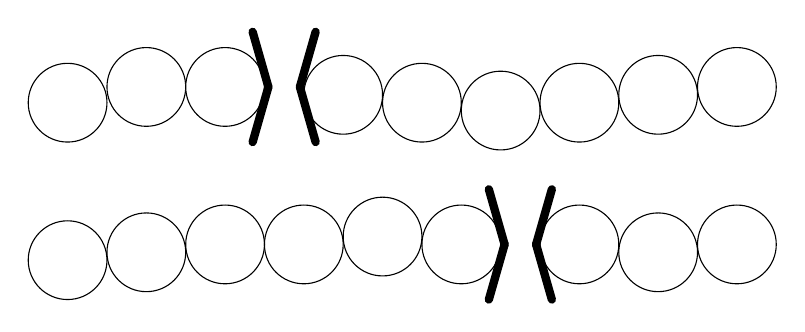
\begin{tikzpicture}
    % Polymer beads
    \foreach \x/\y in {0/0,1/.1,2/.2,3/.2,4/.3,5/.2,6.5/.2,7.5/.1,8.5/.2}
        \draw (\x,\y) circle (5mm);
    % Polymer beads
    \foreach \x/\y in {0/0,1/.2,2/.2,3.5/.1,4.5/0,5.5/-.1,6.5/.0,7.5/.1,8.5/.2}
        \draw[black,fill=white] (\x,2+\y) circle (5mm);
    % Scissors
    \begin{scope}[line width=3,line cap=round]
        % Left scissor
        \draw (5.55,.2) -- (5.35,.9);
        \draw (5.55,.2) -- (5.35,-.5);
        % Right scissor
        \draw (5.95,.2) -- (6.15,.9);
        \draw (5.95,.2) -- (6.15,-.5);
        
        % Left scissor
        \draw (2.55,2.2) -- (2.35,2.9);
        \draw (2.55,2.2) -- (2.35,1.5);
        % Right scissor
        \draw (2.95,2.2) -- (3.15,2.9);
        \draw (2.95,2.2) -- (3.15,1.5);
    \end{scope}
\end{tikzpicture}
